\chapter{ Аналитический раздел}
\label{cha:analysis}

Lorem ipsum dolor sit amet, consectetur adipiscing elit. Integer a mauris consequat, sagittis odio ut, tempor lacus. Donec rhoncus tincidunt ligula, vel egestas turpis vehicula interdum. Phasellus sit amet dignissim metus, quis rutrum metus. Nullam euismod dictum rhoncus. Vivamus bibendum gravida lacus, iaculis consectetur nunc suscipit ac. Aliquam erat volutpat. Nulla laoreet, elit vel lacinia egestas, metus erat sagittis orci, quis vulputate urna tellus ut felis. Morbi sit amet elit auctor, ultrices dui eu, elementum nisi.

\section {Цветовые пространства и модели}
Цветовая модель -- это способ представления цвета в виде кортежа некоторых его независимых между собой характеристик. Как правило, это три составляющие его компоненты, например красный, зелёный и синий или тон, насыщенность и яркость. Цветовое пространство же -- представление цветового множества с помощью такого координатного пространства, что каждая ось преставляет возможные значения одной из компонент кортежа из цветовой модели. Необходимо четко различать цветовые модели и цветовые координатные системы: в первом случае речь идет о способе воспроизведения цветовых ощущений, а во втором — об измерении этих ощущений.

\subsection{CIE RGB}
Цветовая модель $RGB$ -- это аддитивная цветовая модель, в которой красный, зеленый и синий свет суммируются различными способами для воспроизведения широкого спектра цветов. Название модели происходит от инициалов трех аддитивных первичных цветов, красного $R$ , зеленого $G$ и синего $B$.
С помощью этой модели цвет можно представить в виде триплета чисел от 0 до определенного максимального значения, соответственно представляющих долю основных красного, зеленого и синего цветов. Если все компоненты равны нулю, результатом будет черный цвет; если все находятся на максимуме, результат - самый яркий представляемый белый.
Эти диапазоны можно количественно определить несколькими способами:
\begin{enumerate}
	\item От 0 до 1, с любым дробным значением между ними. Это представление используется в теоретических анализах и в системах, которые используют представления с плавающей точкой.
	\item Каждое значение цветового компонента также может быть записано в процентах от 0\% до 100\%.
	\item В компьютерах значения компонентов часто хранятся как целые числа в диапазоне от 0 до 255, диапазон, который может предложить один 8-разрядный байт. Они часто представлены как десятичные или шестнадцатеричные числа.
	\item Высококачественное цифровое графическое оборудование часто может иметь дело с большими целыми диапазонами для каждого основного цвета, например 0..1023 (10 бит), 0..65535 (16 бит) или даже больше, путем расширения 24-бит ( три 8-битных значения) до 32-разрядных , 48-битных или 64-битных единиц (более или менее независимых от размера слова конкретного компьютера )
\end{enumerate}	

\begin{figure}[ht!]
	\centering{ 
		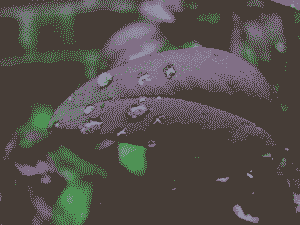
\includegraphics[width=0.4\textwidth]{img/2_bit.png}
		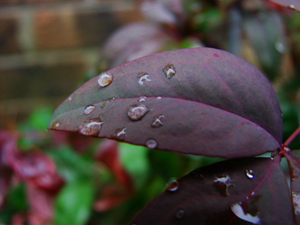
\includegraphics[width=0.4\textwidth]{img/32_bit.png}
		\caption{Cравнение изображений с глубиной цвета 2 бита (слева) и 32 бита (справа)}}
\end{figure}

Количество бит (объём памяти), используемое для хранения и представления цвета при кодировании одного пикселя называют глубиной цвета. 

В начале прошлого века Международная Комиссия по освещению (CIE —
Communication Internationale de l`Eclairage) предприняла попытку  измерить и систематизировать цветовые ощущения человека, вызываемые спектрально-чистыми
цветами, расположенными на всем протяжении видимого спектра: от фиолетового до
красного. Результатом этого эксперимента и стала модель RGB. 

\begin{figure}[ht!]
	\centering{ 
		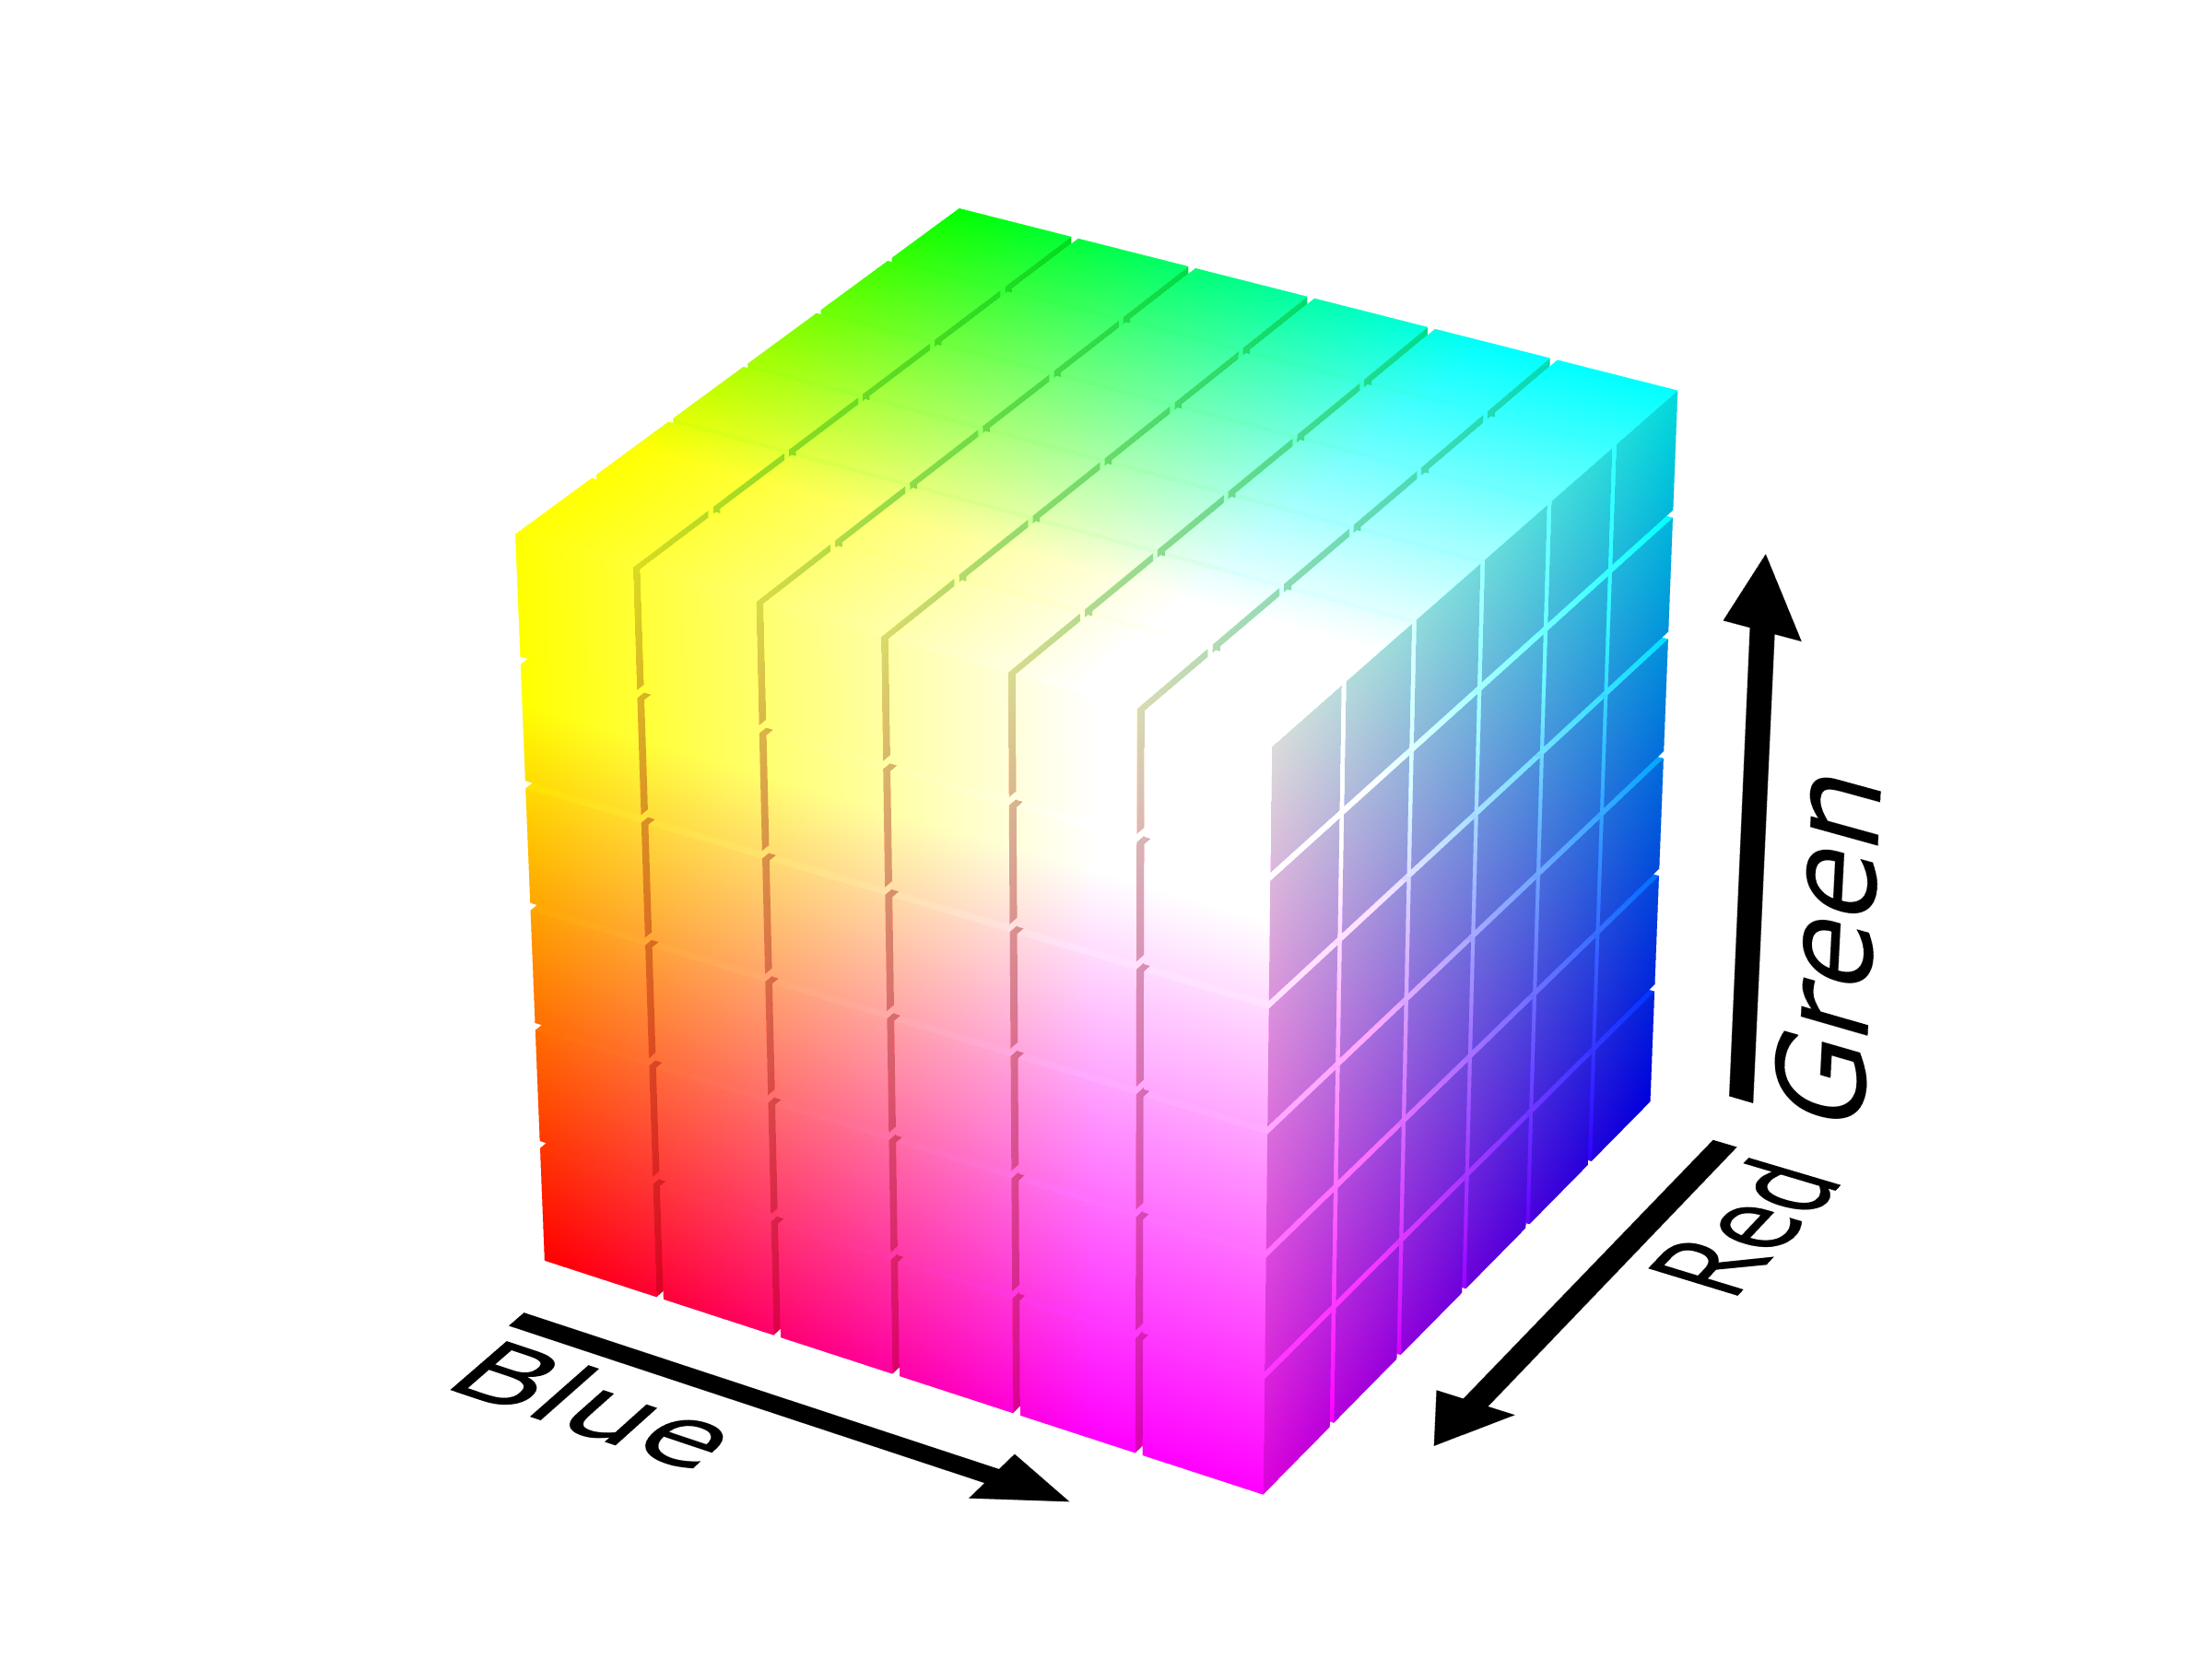
\includegraphics[width=0.4\textwidth]{img/img1.png}
		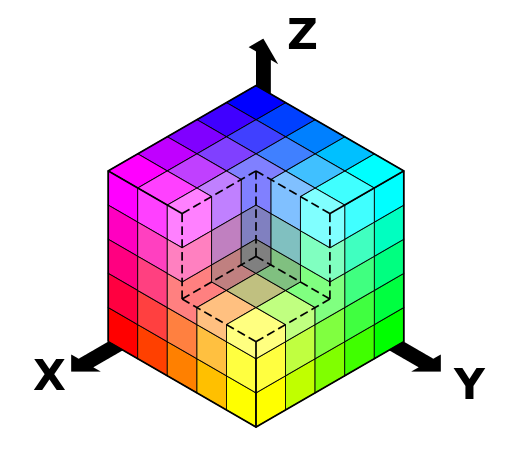
\includegraphics[width=0.4\textwidth]{img/img2.png}
		\caption{Представление цветового куба в пространстве  $RGB$ }}
\end{figure}


\subsection{HSL и HSV}
HSL и HSV являются двумя наиболее распространенными представлениями о цилиндрических или конусных координатах точек в цветовой модели RGB. 

HSL, HLS или HSI  — цветовая модель, в которой цветовыми координатами являются тон (Hue), насыщенность (Saturation) и светлота(Lightness/Intensity). В HSV или HSB светлота заменяется яркостью (Brightness) или значением цвета(Value).

\begin{figure}[ht!]
	\centering{ 
		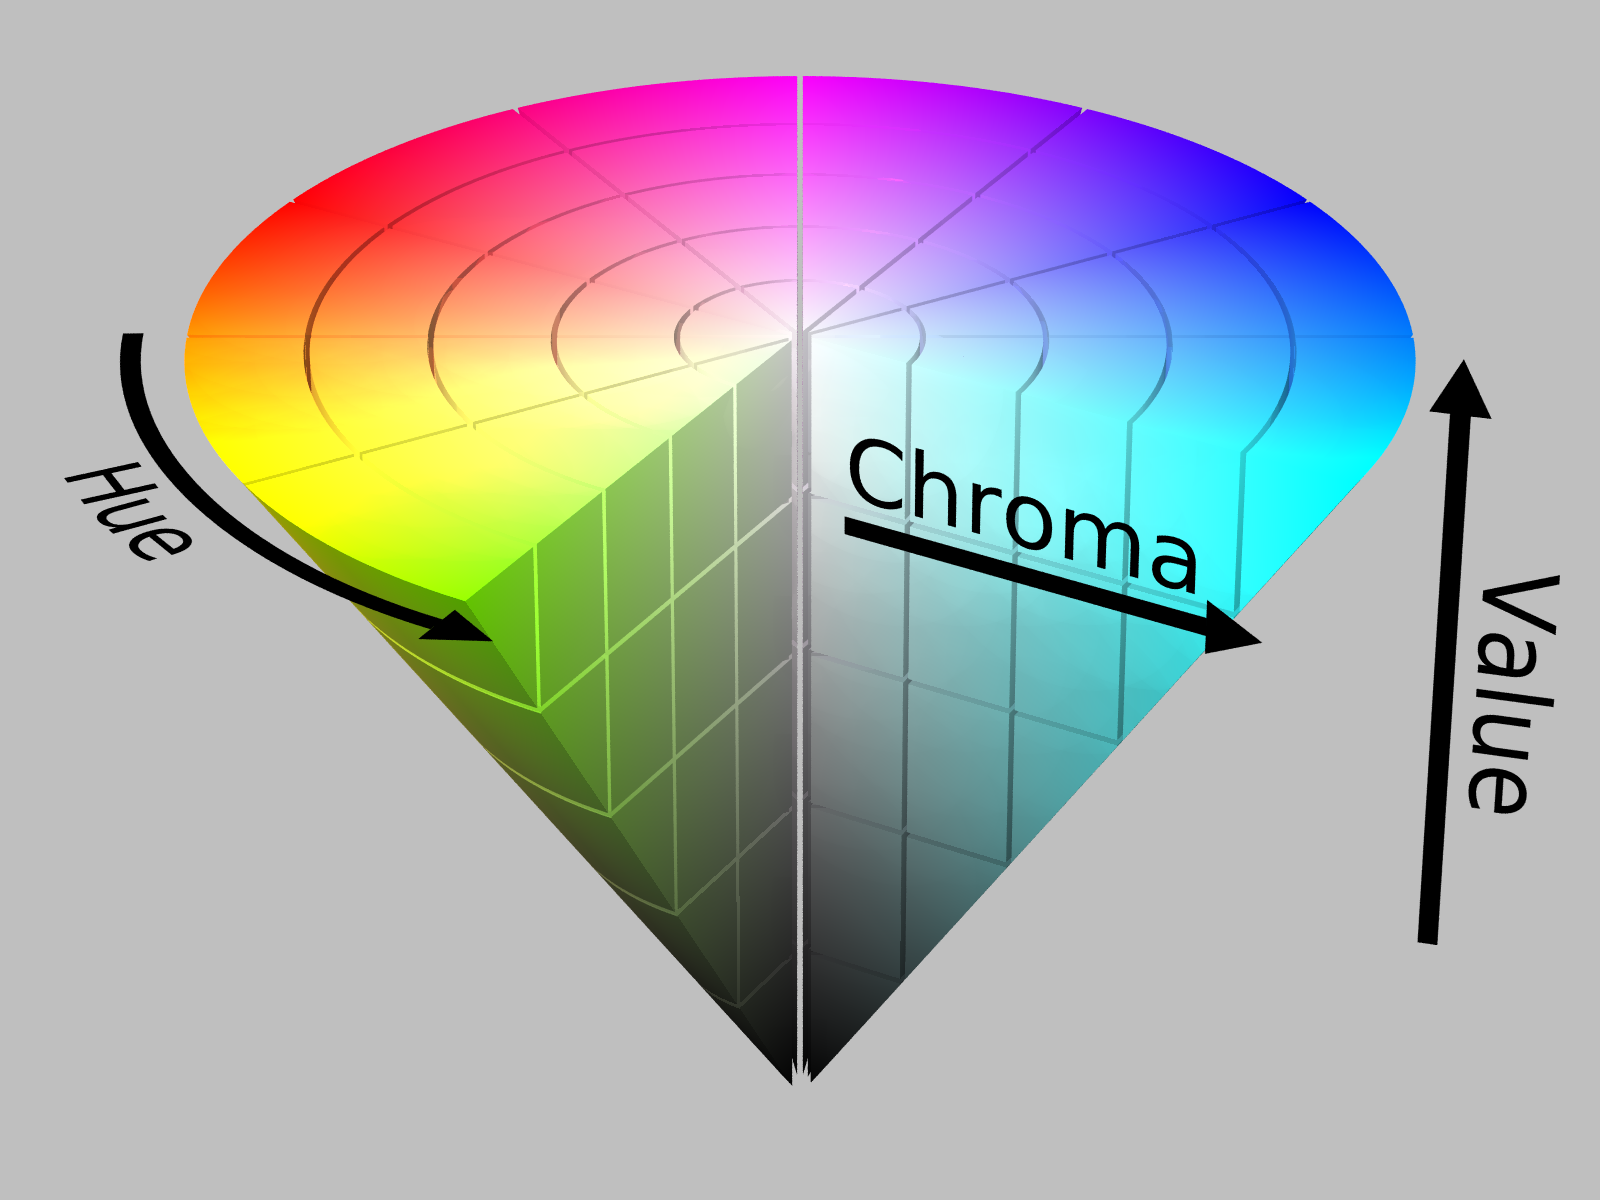
\includegraphics[width=0.4\textwidth]{img/HSV_cone.png}
		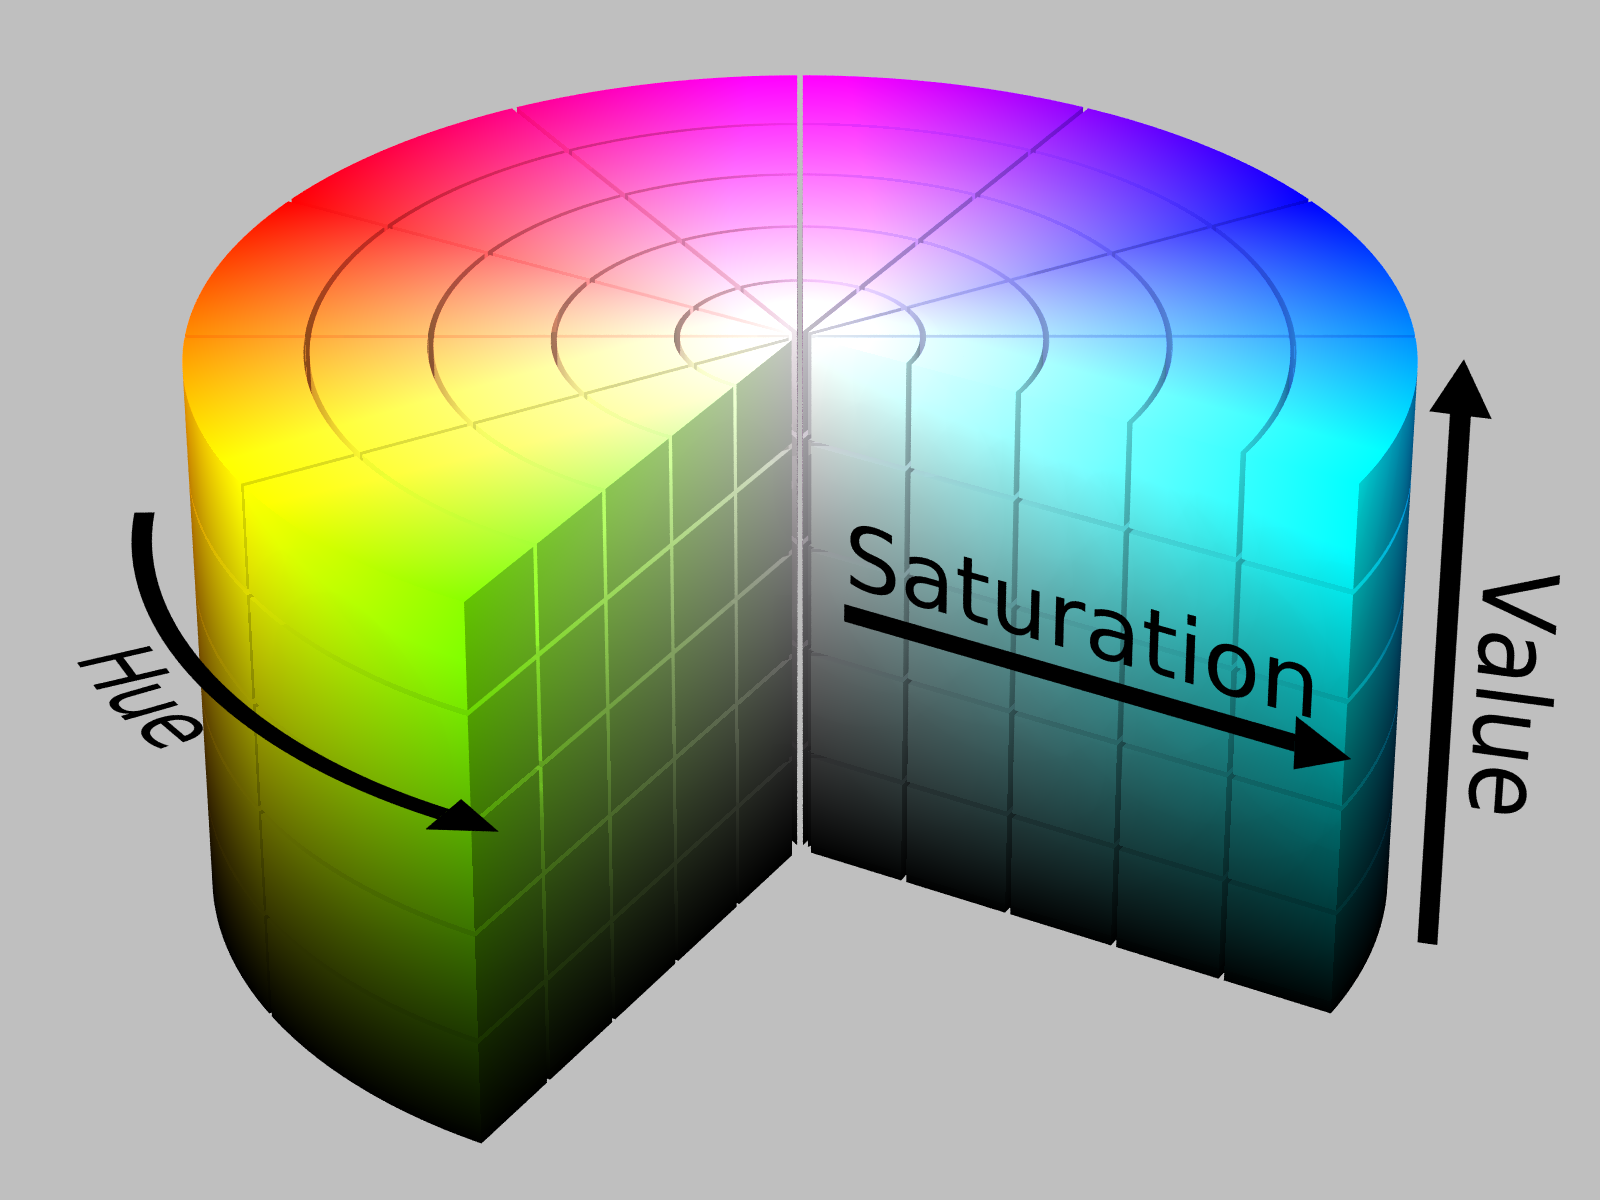
\includegraphics[width=0.4\textwidth]{img/HSV_cylinder.png}
		\caption{Коническое и цилиндрическое представление модели HSV.}}
\end{figure}

Тон (Hue) -- атрибут визуального ощущения, согласно которому область кажется похожей на один из воспринимаемых цветов : красный, желтый, зеленый и синий, или на сочетание двух из них.
Яркость (Brightness) -- атрибут визуального ощущения, согласно которому область излучает больше или меньше света.
Светлота, значение (Lightness, value) -- яркость относительно яркости аналогично освещенного белого.
Цветность (Chroma) -- цветность по отношению к яркости аналогично освещенного белого.
Насыщенность (Saturation) -- красочность цвета относительно его собственной яркости.


\begin{figure}[ht!]
	\centering{ 
		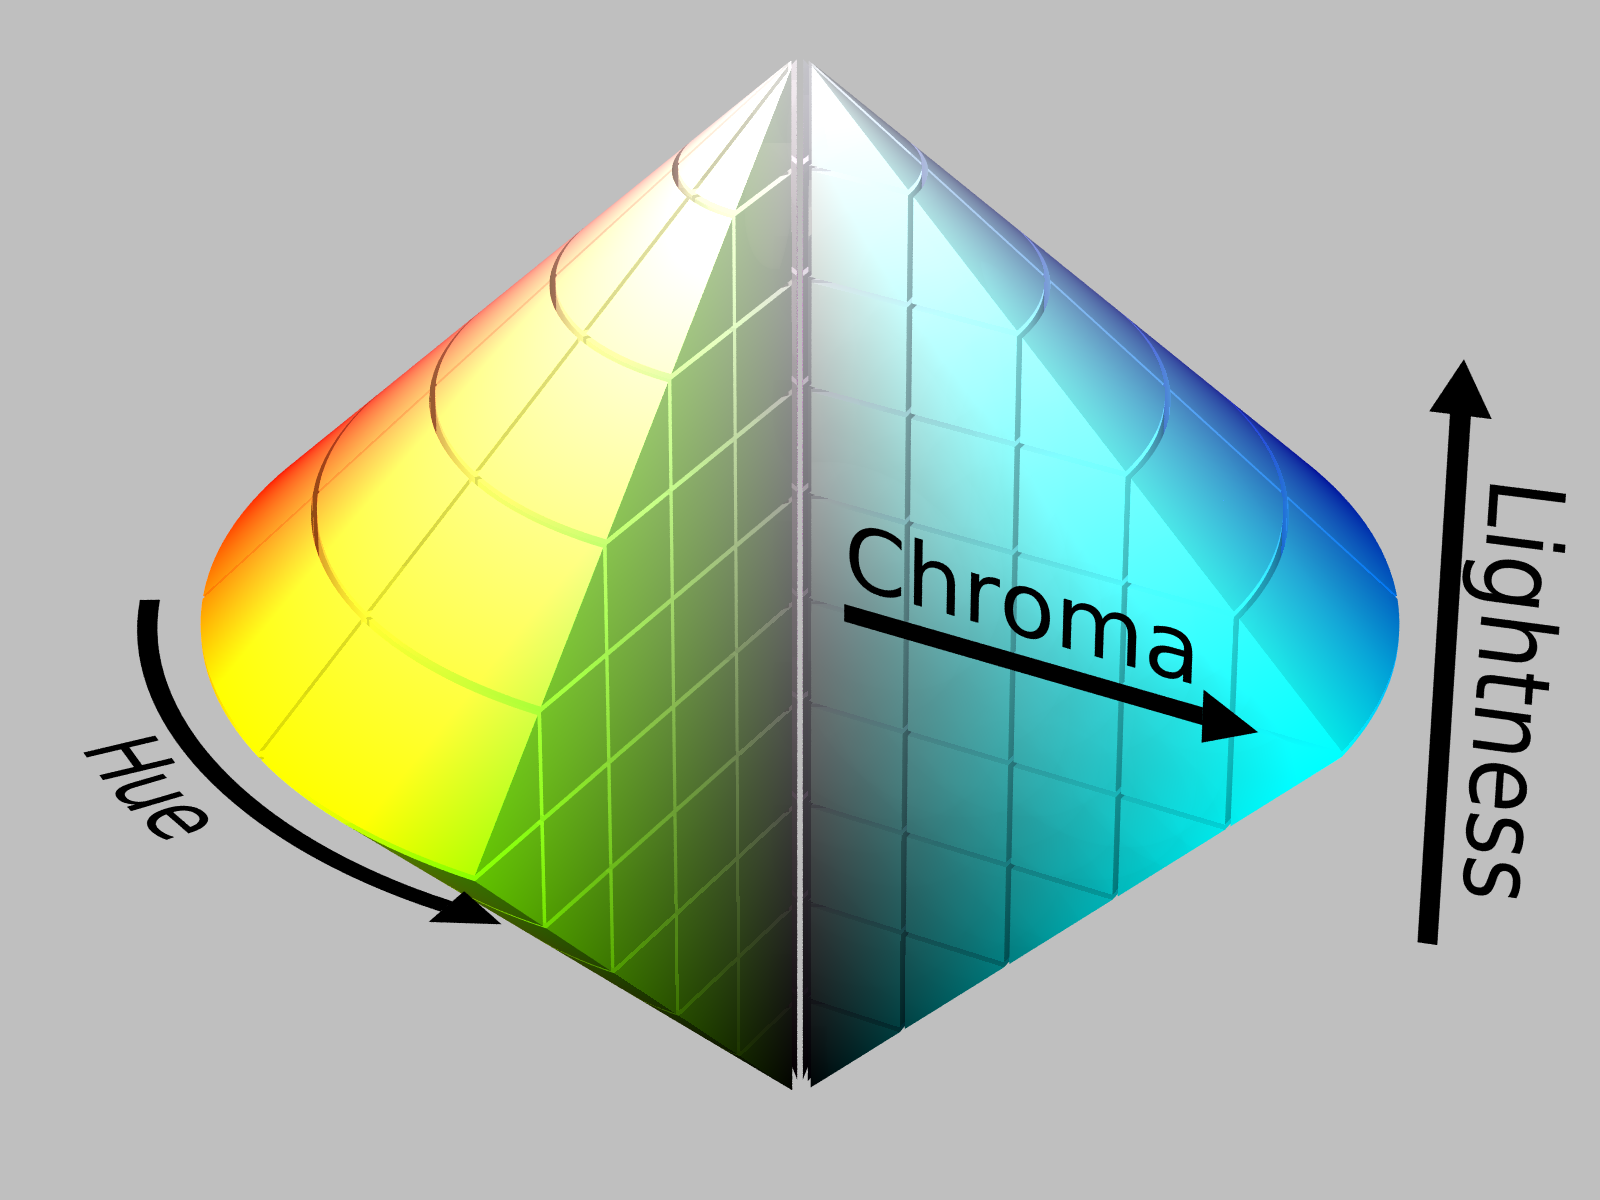
\includegraphics[width=0.4\textwidth]{img/HSL_cone.png}
		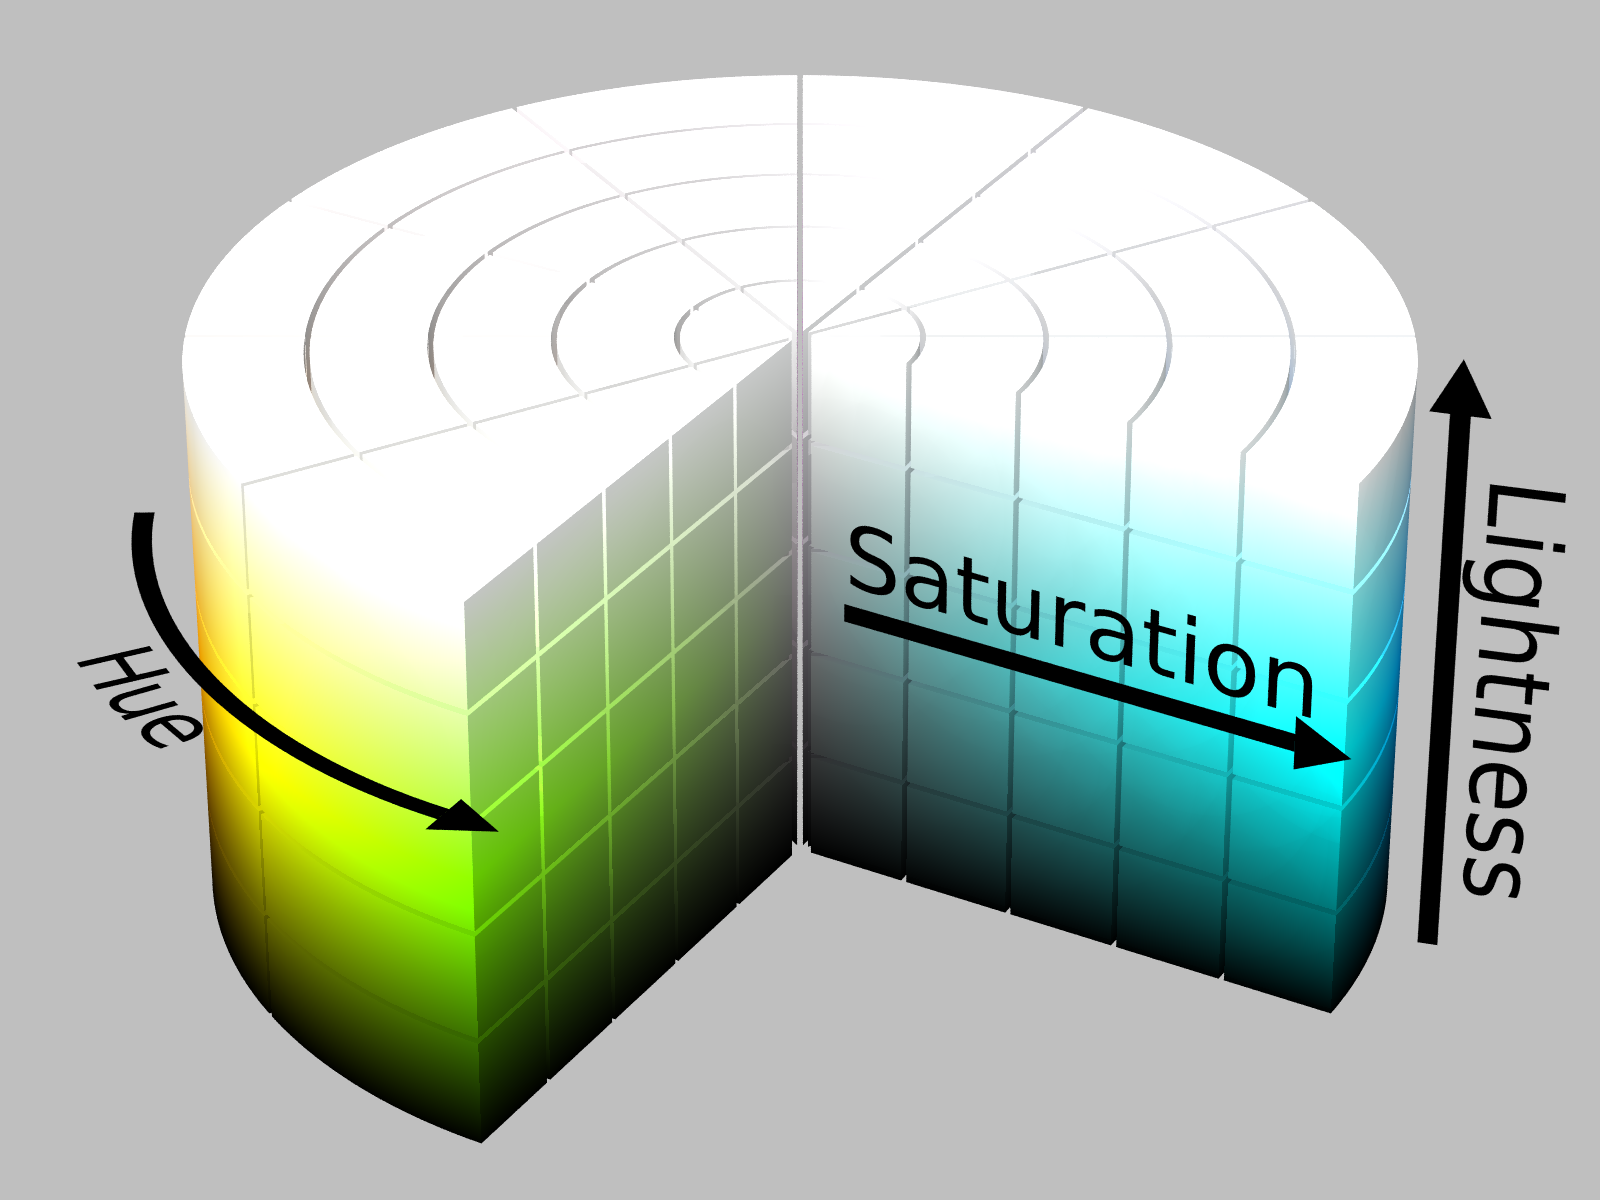
\includegraphics[width=0.4\textwidth]{img/HSL_cylinder.png}
		\caption{Коническое и цилиндрическое представление модели HSL.}}
\end{figure}

HSL и HSV представляют собой цилиндр, где оттенок или тон есть угол, начиная с красного первичного при 0°, проходя через зеленый первичный при 120° и синий первичный при 240°, а затем возвращаясь назад на красный при 360°. Центральная вертикальная ось содержит нейтральные , ахроматические или серые цвета, начиная с черного цвета при освещенности 0 или значения (Value) 0 внизу до белого при яркости 1 или значении (Value) 1, вверху.

В обоих циллиндрах, первичные и вторичные цвета -- красный, желтый , зеленый, голубой , синий и пурпурный  -- и линейные смеси между соседними парами таких цветов, иногда называемые чистыми цветами , расположены вокруг внешнего края цилиндра с насыщенностью 1. Эти насыщенные цвета имеют яркость ½ в HSL, тогда как в HSV они имеют значение 1. Смешивание этих чистых цветов с черными  производными оттенками - не изменяют насыщенности. В HSL насыщенность также не изменяется при тонировании белым, и только смеси и с черным и с белым оттенками имеют насыщенность менее 1. В HSV только тонирование снижает насыщенность.

\begin{figure}[ht!]
	\centering{ 
		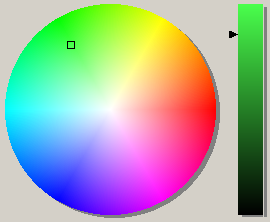
\includegraphics[width=0.4\textwidth]{img/HSV-Slider.png}
		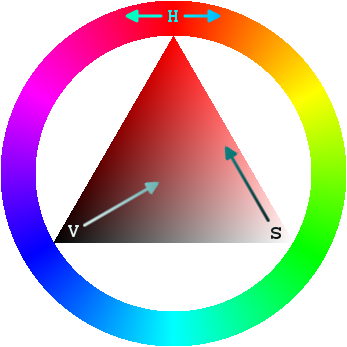
\includegraphics[width=0.4\textwidth]{img/Triangulo_HSV.png}
		\caption{Представление HSV в прикладном ПО.}}
\end{figure}


Оба эти представления широко используются в компьютерной графике, они часто более удобны, чем RGB, но оба они также подвергаются критике за неадекватное разделение атрибутов цветопередачи или отсутствие единообразия восприятия. Перевод из HSV/HSL в RGB довольно сложен. еси  необходимо получить результат смешения двух цветов в одном из этих двух форматов, то лучше произвести все вычисления в RGB, а затем перевести в HSL/HSV по данным формулам: 

RGB → HSV: 

\begin{equation}
 H \in [0°, 360°] 
 \end{equation}
 \begin{equation}
 S,V,R,G,B \in [0,1]
\end{equation}
Пусть $MAX$ — максимальное значение из $R$, $G$ и $B$, а $MIN$ — минимальное из них. Тогда
\begin{equation}
H={\begin{cases} 0°,        if& MAX=MIN \\
	60°\times {\frac  {G-B}{MAX-MIN}}+0°, if& MAX=R, G\geq B \\
	60°\times {\frac  {G-B}{MAX-MIN}}+360°, if& MAX=R, G < B \\
	60°\times {\frac  {B-R}{MAX-MIN}}+120°, if& MAX=G \\
	60°\times {\frac  {R-G}{MAX-MIN}}+240°, if& MAX= B \\
	\end{cases}}
\end{equation}

 \begin{equation}
S={\begin{cases} 0, if&{\displaystyle MAX=0} \\
else&{\displaystyle 1-{\dfrac {MIN}{MAX}}}  
	\end{cases}}	
\end{equation}
 \begin{equation}
V=MAX
\end{equation}

RGB → HSL:\\
Пусть $MAX$ — максимальное значение из $R$, $G$ и $B$, а $MIN$ — минимальное из них. Тогда $H$ определяется аналогично модели HSV.
 \begin{equation}
L=\frac{1}{2}(MAX+MIN)
\end{equation}
 \begin{equation}
S={\begin{cases} 0, if  L = 0 \vee MAX = MIN \\
	 \frac{MAX-MIN}{1-|1-(MAX+MIN)|}
	\end{cases}}
\end{equation}

\section{Методы смешивания цветов}
 Смешение цветов - это синтез нового цвета на основе двух других.  Видимые в естественных условиях цвета, как правило, являются результатом
 смешения спектральных цветов.
 Существует два различных типа смешения цветов. Это аддитивное (слагательное) смешение и субтрактивное (вычитательное) смешение.
 
\subsection{Аддитивный синтез}
Аддитивный цвет - это цвет, созданный путем смешивания нескольких различных цветов света, причем оттенки красного , зеленого и синего являются наиболее распространенными основными цветами, используемыми в аддитивной цветовой системе.Автором теории аддитивного синтеза считают Джеймса Клерка Максвелла, вдохновленного теории Юнга-Гельмгольца о трехцветном цветовом зрении.

\begin{figure}[ht!]
	\centering{ 
		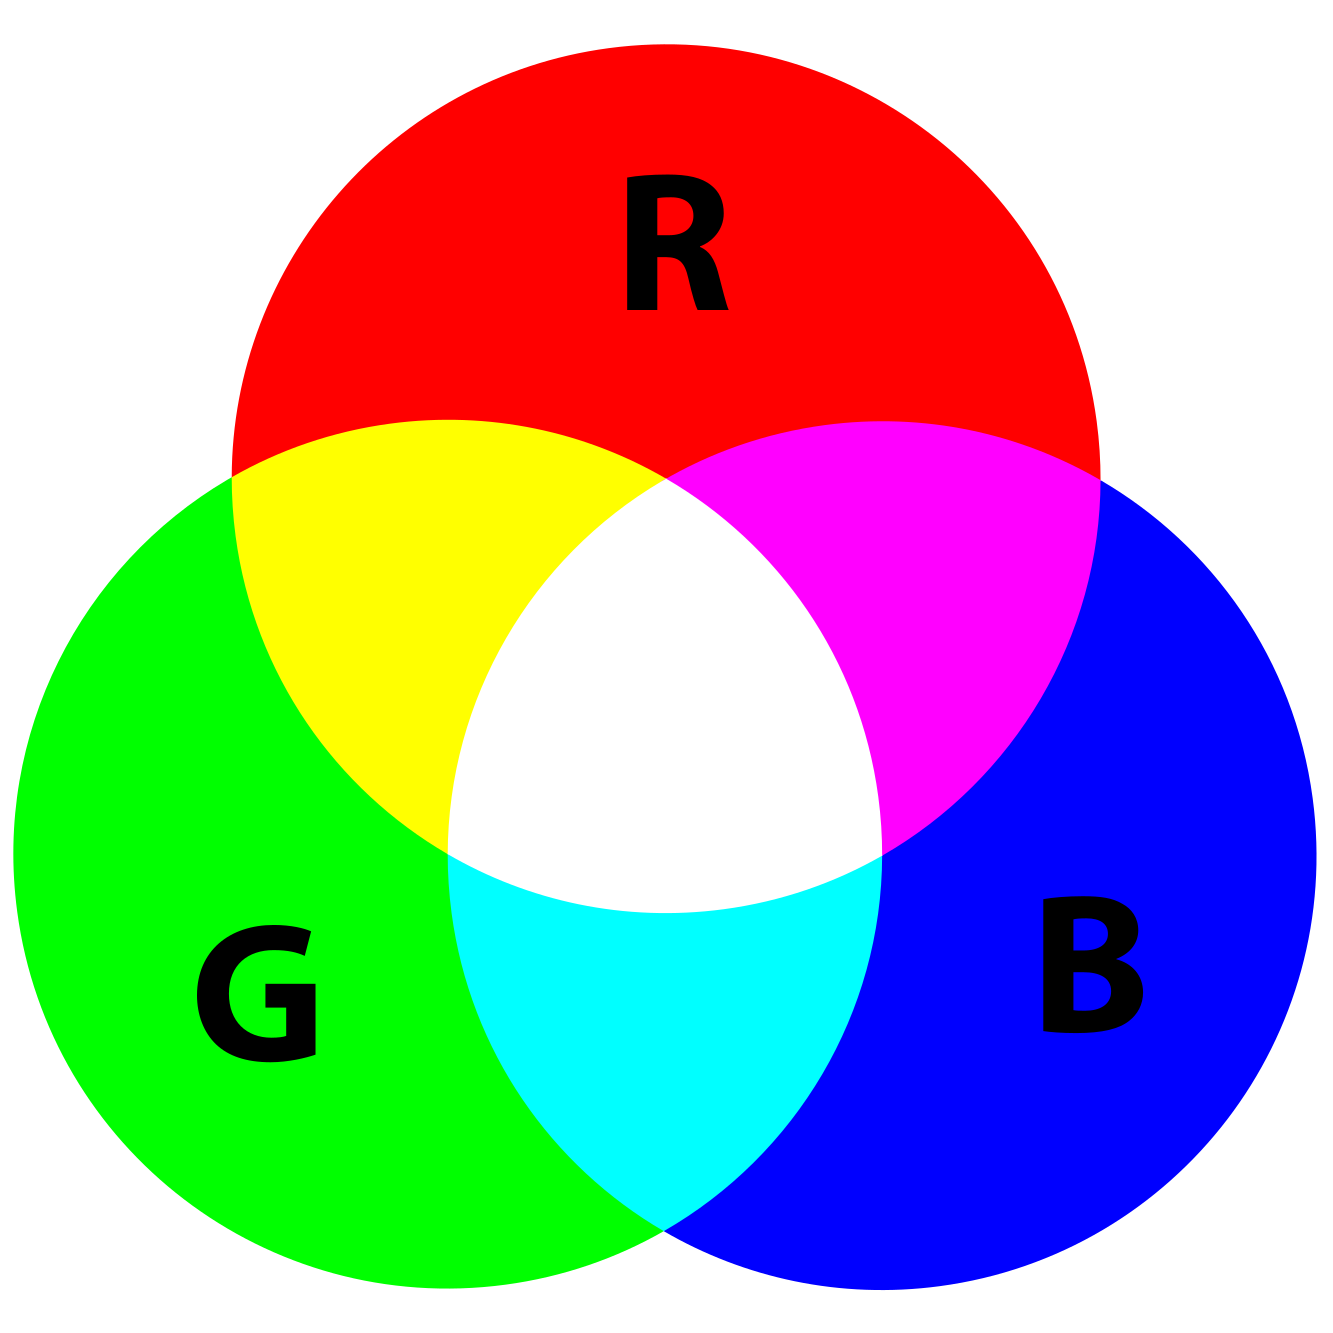
\includegraphics[width=0.45\textwidth]{img/AdditiveColor.png}
		\caption{Аддитивный синтез: первичные красный, зеленый и синий в смешении попарно дают вторичные цвета, а все три дают белый цвет}}
\end{figure}

Существует большая разница между чистым спектральным желтым светом с длиной волны около 580 нм и смесью красного и зеленого света. Тем не менее, оба стимулируют наши глаза подобным образом, поэтому мы не обнаруживаем эту разницу, и оба являются желтым светом для человеческого глаза. 


Компьютерные мониторы и телевизоры являются наиболее распространенными примерами аддитивного синтеза. Каждый пиксель на большинстве типов цветных видеодисплеев состоит из красных, зеленых и синих субпикселей, свет из которых сочетается в разных пропорциях, чтобы производить все остальные цвета, а также белые и оттенки серого. Цветные субпикселы не перекрываются на экране, но при просмотре даже с небольшого  расстояния они перекрываются и смешиваются на сетчаткой глаза, производя тот же результат, что и внешнее наложение.


\subsection{Субтрактивный синтез}
Субтрактивный синтез объясняет смешение ограниченного набора красителей, красок, пигментов или натуральных красителей для создания более широкого диапазона цветов, каждый из которых является результатом частичного или полного вычитания (то есть, поглощения) некоторых длин волн света. Цвет, который отображается на поверхности, зависит от того, какие части видимого спектра не поглощаются и ,следовательно , остаются видимыми.

\begin{figure}[ht!]
	\centering{ 
		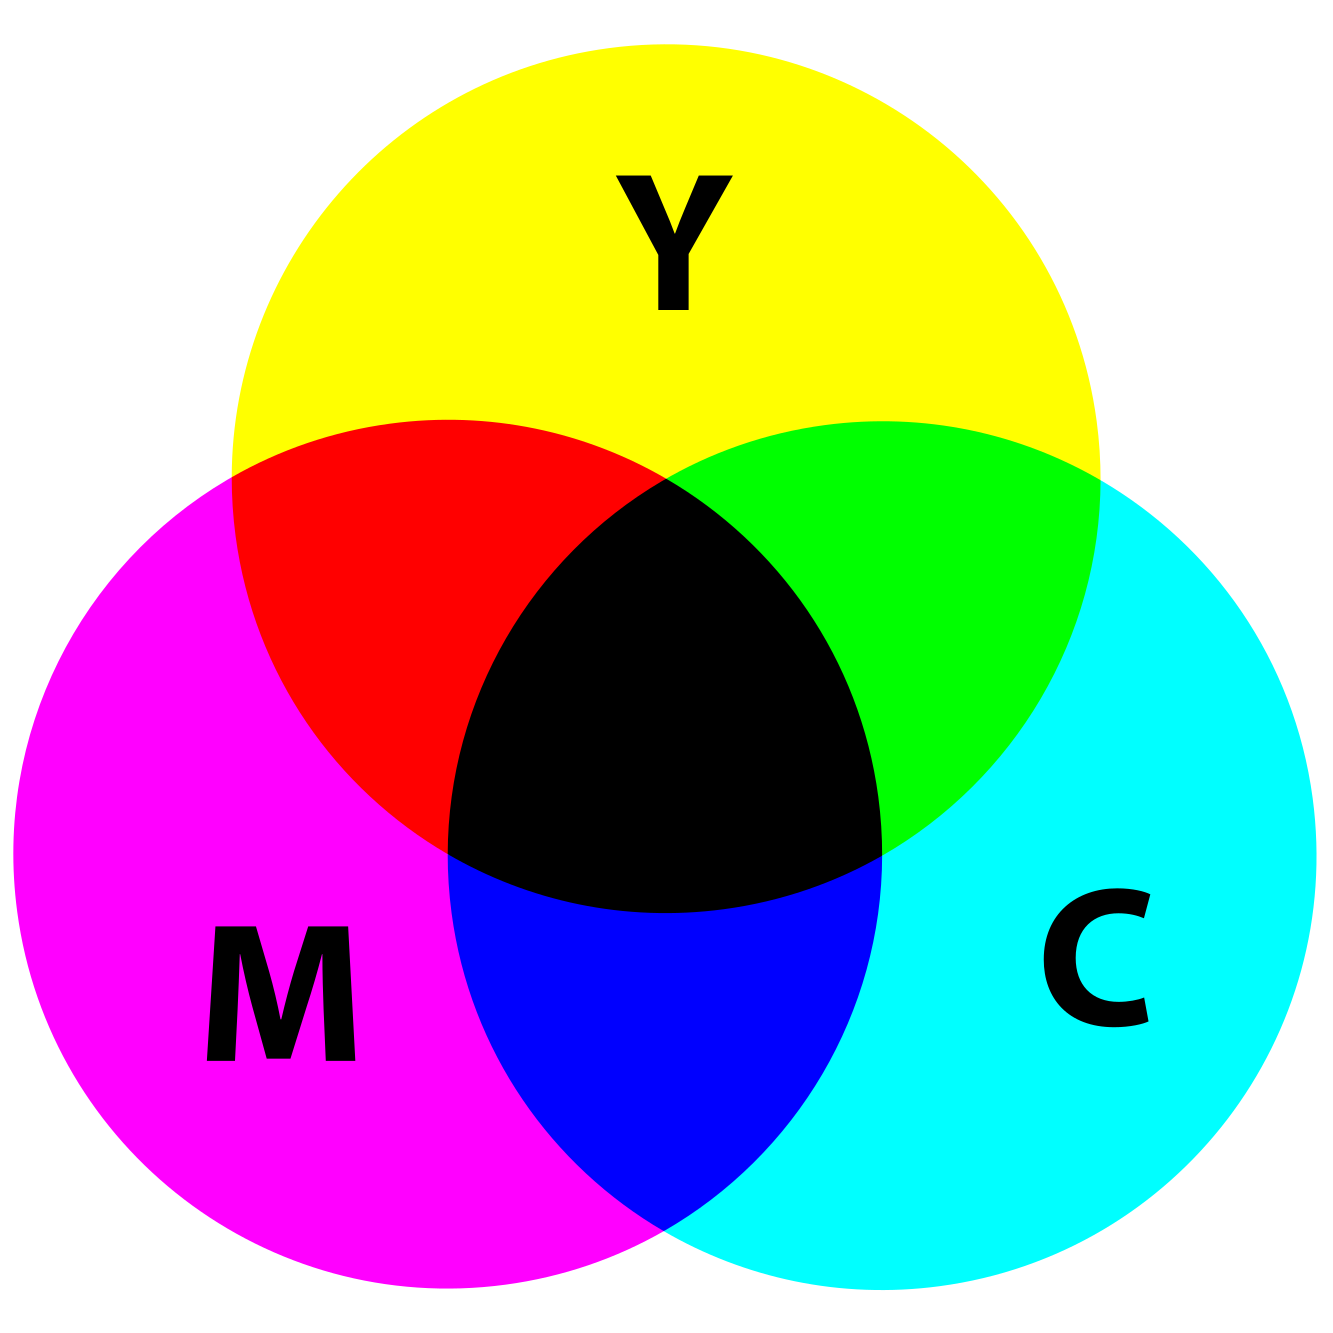
\includegraphics[width=0.45\textwidth]{img/SubtractiveColor.png}
		\caption{Субтрактивный синтез, где роль первичных цветов играют   голубой(cyan), пурпурный(magenta) и жёлтый.}}
\end{figure}

\section{Альфа-канал}
Термин «альфа-канал» впервые введён в оборот Алви Смитом в конце 1970-х гг. и детально проработан в статье Томаса Портера и Тома Даффа 1984 года.

Альфа-каналом назовём компонету цветовой модели, представляющую коэффициент смешивания для управления линейной интерполяцией цветов переднего плана и фона. Такую компоненту будем обозначать $\alpha$, $\alpha = 0$ будем сопоставлять с полной прозрачностью пикселя, а $\alpha=1 (255)$ -- с полной непрозрачностью. \cite{bib2} 

Если в изображении используется альфа-канал, доступны два общих представления: прямая (непривязанная) $\alpha$ и премультиплексированная (ассоциированная) $\alpha$. С прямой $\alpha$ компоненты RGB представляют цвет объекта или пикселя, не обращая внимания на его непрозрачность. С премультиплексированной $\alpha$ компоненты RGB представляют цвет объекта или пикселя, скорректированный на его непрозрачность путем умножения. Такое представление обладает рядом преимуществ: 
\begin{enumerate}
	\item премультиплексированное $\alpha$-смешивание является ассоциативным.
	\item интерполяция и фильтрация дают правильные результаты. При интерполяции или фильтрации изображений без предварительно умноженной $\alpha$ с резкими границами между прозрачными и непрозрачными областями  может привести к границам цветов, которые не были видны в исходном изображении. Ошибки также возникают в областях полупрозрачности, потому что компоненты RGB неправильно взвешены, что приводит к некорректному взвешиванию цвета более прозрачных пикселей.
	\item уникальное представление для прозрачных пикселей. Представления цветов в виде (1, 0.5, 1, 0) невозможны.
\end{enumerate}


\subsection{RGBA}
RGBA -- цветовое пространство RGB c альфа-каналом. Четверка $(R, G, B, \alpha)$ говорит о том, что пиксель покрыт цветом $(\alpha R, \alpha G, \alpha B)$. 

\begin{figure}[ht!]
	\centering{ 
		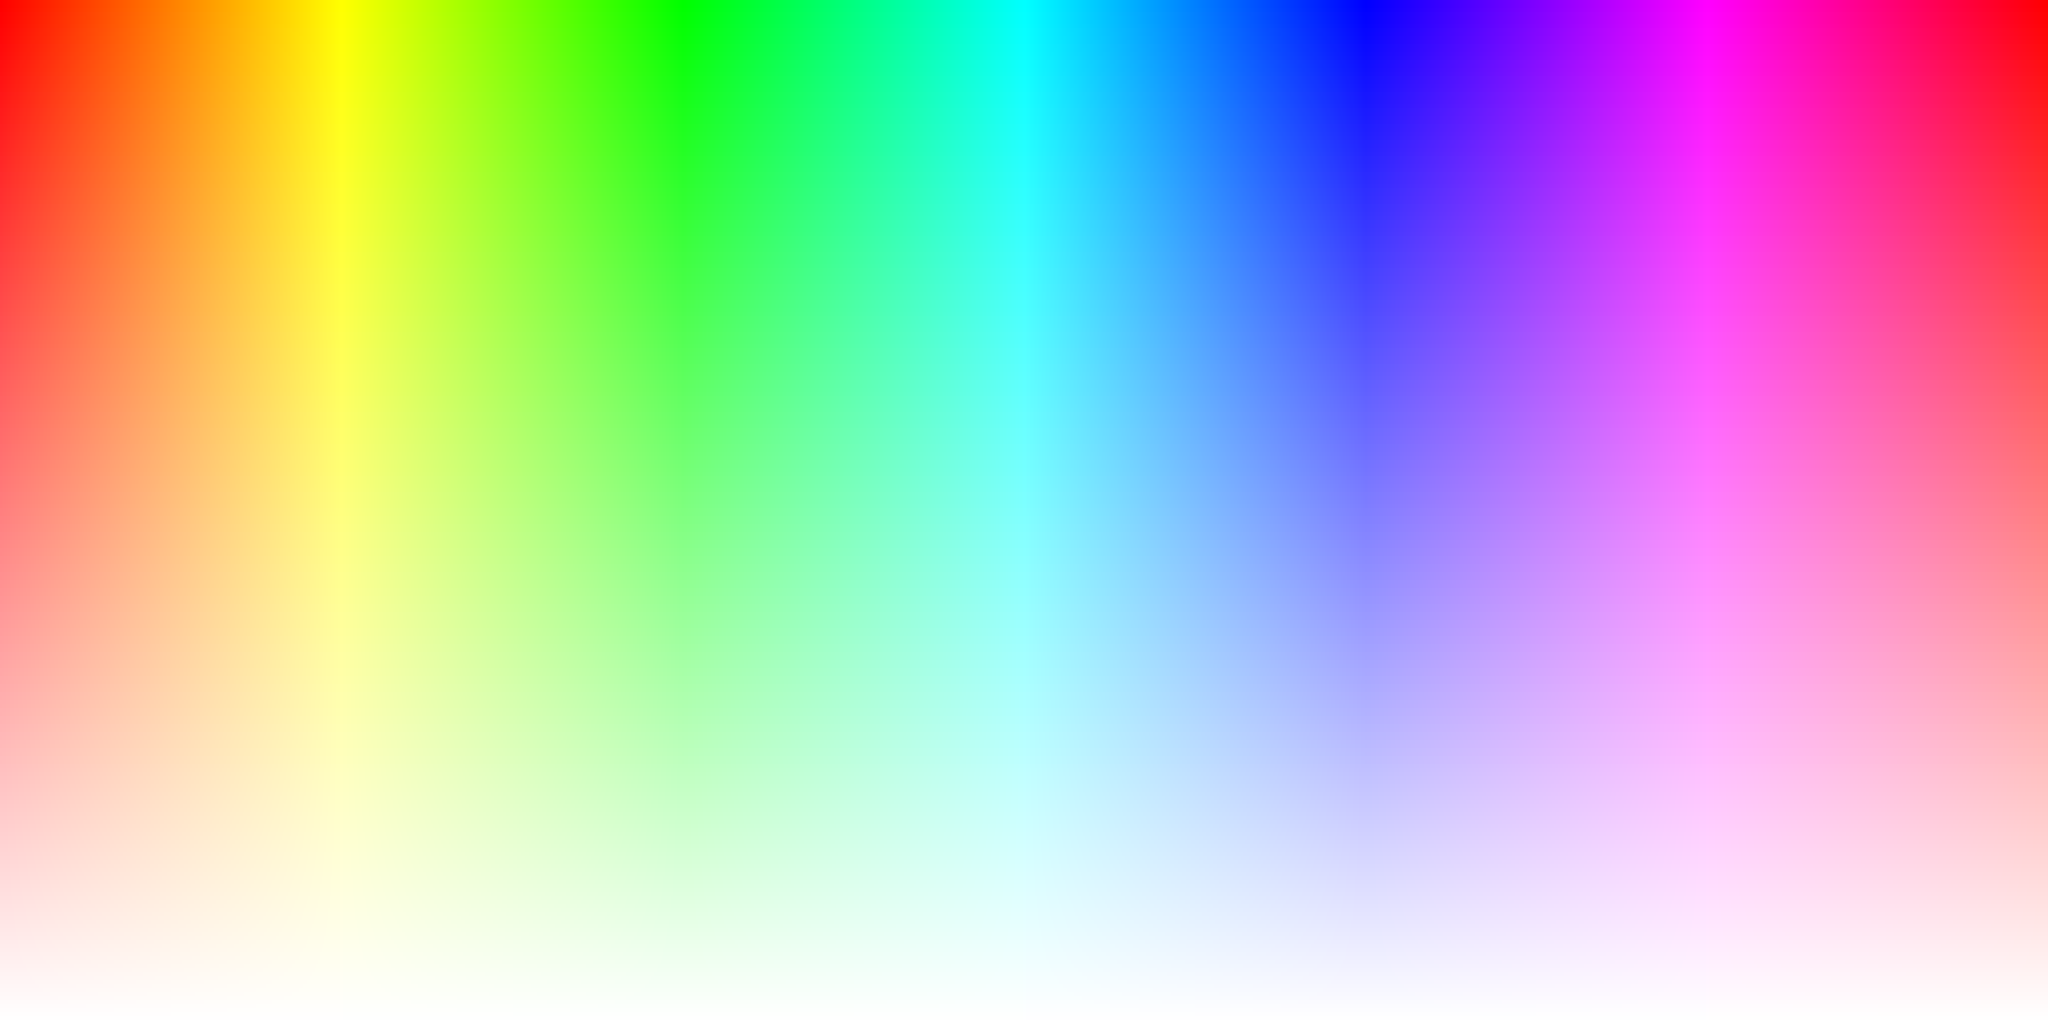
\includegraphics[width=0.5\textwidth]{img/img6.png}
		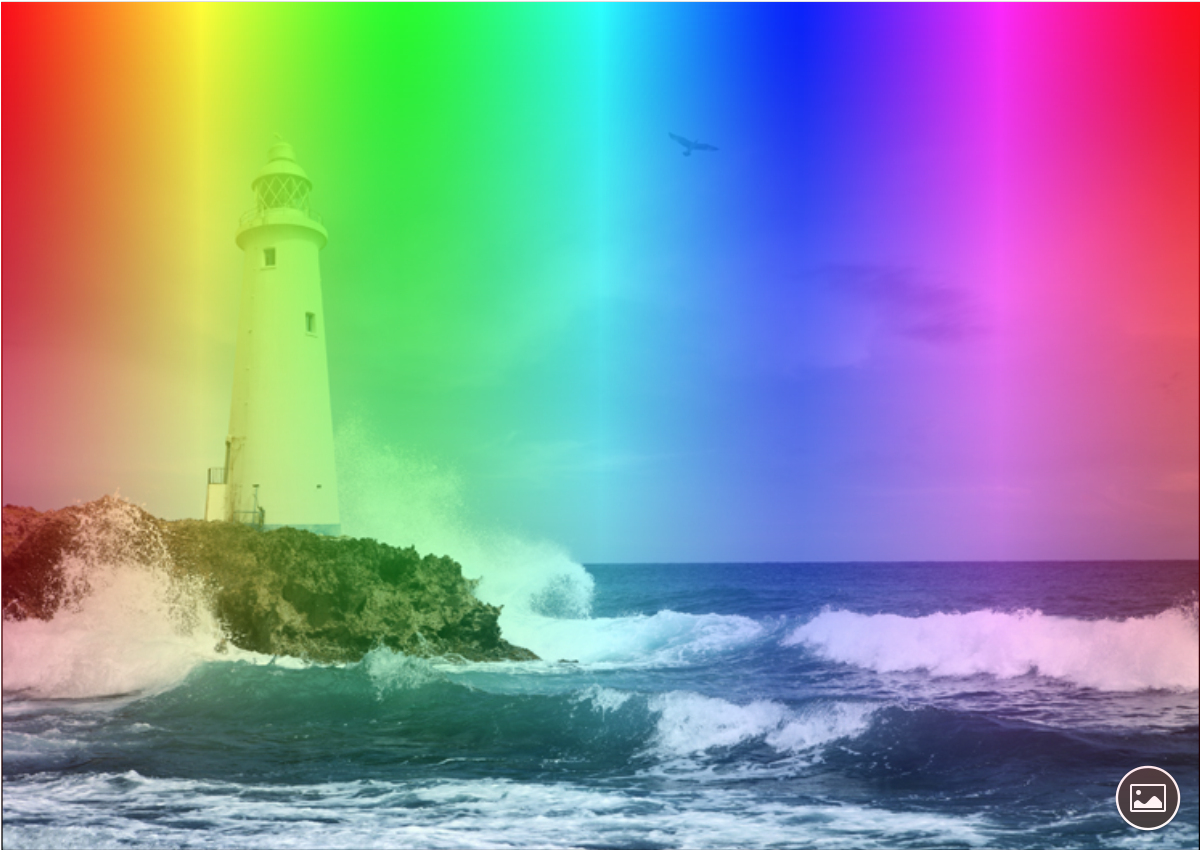
\includegraphics[width=0.45\textwidth]{img/img7.png}
		\caption{Альфа-канал первого изображения меняется от 1 до нуля сверху вниз. На втором изображении совмещены изображения маяка и предыдущее изображение.}}
\end{figure}

Важно различать два ключевых пиксельных представления:
непрозрачный черный  (0,0,0,1) и полностью поозрачный пиксел  (0,0,0,0).


\section{Альфа-смешение}
Альфа-смешивание -- это смешивание двух и более цветов с учетом их альфа-каналов. Альфа-смешивание представляет собой выпуклую комбинацию из двух цветов, обеспечивающую эффект прозрачности в компьютерной графике. Стоит отметить несколько граничных случаев. Если цвет переднего плана полностью прозрачный, смешанный цвет будет цветом фона. И наоборот, если он полностью непрозрачен, смешанный цвет будет цветом переднего плана.
Прозрачность может варьироваться, и в этом случае смешанный цвет вычисляется как средневзвешенное значение цветов переднего плана и фона.

\subsection{Расчёт результирующего цвета}
Пусть пиксель А имеет $\alpha = \alpha_{A}$ и "чистый" цвет $A$, а пиксель B  -- $\alpha = \alpha_{B}$ и "чистый" цвет $B$. Таким образом,  результирующий цвет каждого отдельного взятого пикселя будет равен

\begin{equation}
C_{A} = \alpha_{A}A 
\end{equation}
\begin{equation}
C_{B} = \alpha_{B}B
\end{equation}

Если асссоциировать $\alpha$ с процентным покрытием пикселя равномерным пикселем \cite{bib8}, то пиксель А может покрыть своей непрозрачной составляющей не более, чем $1- \alpha_{B}$ процентов пикселя.  Отсюда следует, что результирующий цвет таков

\begin{equation}
C_{O} = \alpha_{B}B + (1- \alpha_{B})\alpha_{A}A = C_{B} + (1- \alpha_{B})C_{A},
\end{equation}
что является выпуклой комбинацией A и B.

Стоит заметить, что данный результат может оказаться неправильным в случае, если характеристики  А и В совпадают.  

Можно вывести формулу (1.35) более строго. 

\subsection{Аналитический вывод результирующего цвета}
Обозначим оператор $AoverB$ как $A \oplus B$. 
Первое предположение состоит в том, что в случае, когда фон непрозрачен (т.е. $\alpha _ {B} = 1$), Оператор $\oplus$ представляет собой выпуклую комбинацию из A и B:
\begin{equation}
O= \alpha_{A}A + (1- \alpha_{A})B
\end{equation}
Второе предположение состоит в том, что оператор должен удовлетворять ассоциативному правилу:
\begin{equation}
(A \oplus B) \oplus C = A \oplus (B \oplus C)
\end{equation}
Пусть A и B имееют переменную прозрачность, а C непрозрачен. Тогда нужно найти
\begin{equation}
O = A \oplus B
\end{equation}
Из (1.37) и (1.38):
\begin{equation}
O \oplus C = A \oplus (B \oplus C)
\end{equation}
Т.к. С непрозрачен, то и В $\oplus$ C непрозрачен. , поэтому в приведенном выше уравнении каждый  $\oplus$ оператор можно записать в виде выпуклой комбинации:
\begin{equation}
\alpha_{O}O + (1 - \alpha_{O}) C = \alpha_{A}A + (1 - \alpha_{A})(\alpha_{B} + (1 - \alpha_{B})C) \\
= \alpha_{A}A + (1 - \alpha_{A})\alpha_{B}B + (1-\alpha_{A})(1-\alpha_{B})C
\end{equation}
Отсюда видно, что это представляет собой уравнение вида $ X_{0} + Y_{0} C = X_{1} + Y_{1} C$, установив  $X_{0} = X_{1}$, а также $Y_{0} = Y_ {1}$ мы получаем

\begin{equation}
\alpha_{O} = 1 - (1 - \alpha_{A})(1 - \alpha_{B}) =  \alpha_{A} + \alpha_{B}(1-\alpha_{A})
\end{equation}

\begin{equation}
O = \frac{\alpha_{A}A + (1-\alpha_{A})\alpha_{B}B}{\alpha_{O}}
\end{equation}

Еще более компактное представление дается, замечая, что $(1- \alpha_{A}) \alpha_{B} = \alpha_{O} - \alpha_{A}$:

\begin{equation}
O = \frac{\alpha_{A}}{\alpha_{O}}A + (1-\frac{\alpha_{A}}{\alpha_{O}})B
\end{equation}

Интересно также отметить, что оператор  $\oplus$ удовлетворяет всем требованиям некоммутативного моноида, где единичный элемент $е$ выбирается таким образом, что  $e\oplus A = A \oplus e = A$. Т.е. единичный элемент может быть любым кортежем $\langle C, \alpha \rangle$ c $\alpha = 0$.

Если же используется премультиплексированная $\alpha$, то уравнение (1.42) примет вид, аналогичный (1.35): 

\begin{equation}
C_{O} = C_{A} + (1-\alpha_{A})C_{B}
\end{equation}

\subsection{Сравнение премультиплексированной  $\alpha$ и прямой $\alpha$}
Премультиплексированное представление обладает рядом преимуществ: 
\begin{enumerate}
	\item премультиплексированное $\alpha$-смешивание является ассоциативным.
	\item интерполяция и фильтрация дают правильные результаты. При интерполяции или фильтрации изображений без предварительно умноженной $\alpha$ с резкими границами между прозрачными и непрозрачными областями  может привести к границам цветов, которые не были видны в исходном изображении. Ошибки также возникают в областях полупрозрачности, потому что компоненты RGB неправильно взвешены, что приводит к некорректному взвешиванию цвета более прозрачных пикселей.
	\item уникальное представление для прозрачных пикселей. Представления цветов в виде (1, 0.5, 1, 0) невозможны.
\end{enumerate}
Использование же прямой $\alpha$ создает ряд проблем. Рассмотрим их подробнее.
 
\subsection{Проблема повторной композиции и \\ накопление погрешности}
Данная проблема проявляется при композиции/смешивании трех и более цветов, используя результат предыдущих двух цветов.

Пусть пиксель K является результатом для  J $\oplus$ I. Предположим, что мы хотим выполнить L $\oplus$ K, используя прямую $\alpha$.

\begin{equation}
K = \frac{\alpha_{J}J + (1-\alpha_{J})\alpha_{I}I}{\alpha_{K}}
\end{equation}

\begin{equation}
L \oplus K = \frac{\alpha_{L}L + (1-\alpha_{L})\alpha_{K}K}{\alpha_{L \oplus K}}
\end{equation}

Как видно из вышепредставленных формул, мы все время делим и умножаем на $\alpha_{K}$, что сильно снижает производительность и эффективность. При использовании целочисленного представления цветов это приводит к большим неточностям при даже небольшом наслаивании пикселей. Также при $\alpha = 0$ это приводит к ошибке деления на ноль. Сама $\alpha = 0$ приводит к неоднозначности: пиксель (1, 1, 1, 0) может существовать так же, как и (1, 1, 1, 0). Во-первых, это лишено физического смысла. Во-вторых, при смешивании это может приводить к лишним вычислениям, когда пиксель не будет вносить вклад в результирующий цвет, но будет просчитан, т.к. будет обладать цветом. 

\subsection{Конкретизация формул для альфа-смешения}
Пусть $src$ смешивается с $dst$. Результирующий цвет обозначим как $out$.
Тогда, используя премультиплексированную $\alpha$: 

\begin{equation}
\begin{cases} out_{A} = src_{A} + dst_{A}(1-src_{A}) \\
out_{RGB} = src_{RGB} + dst_{RGB}(1-src_{A})
\end{cases}
\end{equation}

Следует заметить, что под $out_{RGB}$  подразумевается кортеж значений $\langle R, G, B\rangle$, где $R, G, B \in [0, 255]$.

\section{Анализ существующих технологии оптимизации вычисления}
Оптимизация на низком уровне чаще всего дает больший прирост в скорости приложения, чем ручная оптимизация. Крупные компании-производетели процессоров, такие как Intel или AMD, работают над технологиями, позволяющими использовать определенные команды процессора для более эффективной работы с памятью. Также существует тенденция на перенос некоторых объемов вычислений на GPU. 

\subsection{CUDA}
CUDA – это программно-аппаратная архитектура параллельных вычислений от NVIDIA, позволяющая существенно увеличить вычислительную производительность благодаря использованию GPU (графических процессоров) фирмы NVIDIA.

CUDA  позволяет программистам реализовывать на специальном упрощённом диалекте языка программирования Си алгоритмы, выполнимые на графических процессорах NVIDIA, и включать специальные функции в текст программы на Си. Архитектура CUDA даёт разработчику возможность по своему усмотрению организовывать доступ к набору инструкций графического ускорителя и управлять его памятью.

Разработчики программного обеспечения, ученые и исследователи широко используют CUDA в различных областях, включая обработку видео и изображений, вычислительную биологию и химию, моделирование динамики жидкостей, восстановление изображений, полученных путем компьютерной томографии, сейсмический анализ, трассировку лучей и многое другое.

Достоинствами CUDA является огромный прирост скорости выполнения расчётов по сравнению с расчетами на центральном процессоре компьютера. Для некоторых задач ускоррение может измеряться сотнями за счёт более эффективные транзакций между памятью центрального процессора и видеопамятью.

Недостатками является сложность программирования для CUDA (хотя производитель утверждает обратное), привязка к картам NVIDIA, и, как вследствие, отсутствие переносимости между архитектурами.


\subsection{SSE}
\subsection{AVX}
\subsubsection{Различия AVX и AVX2}
\subsubsection{Необходимые условия использования технологии AVX2}
\subsection{Распараллеливания вычислений}
\section{Применение AVX2 для оптимизации смешения цветов}
\subsection{Достоинства технологии}
\subsection{Недостатки технолгии}




%%% Local Variables:
%%% mode: latex
%%% TeX-master: "rpz"
%%% End:
